\documentclass[30pt, a0paper, portrait, margin=0mm, innermargin=15mm,
               blockverticalspace=15mm, colspace=15mm, subcolspace=8mm]{tikzposter} 

% Change font     
\renewcommand{\familydefault}{\sfdefault}

\definecolor{mycol}{HTML}{326E77}
\definecolorstyle{myColorStyle}{
  \colorlet{colorOne}{darkgray}
  \colorlet{colorTwo}{gray}
  \colorlet{colorThree}{gray}
}{
  % Background Colors
  \colorlet{backgroundcolor}{colorTwo!50}
  \colorlet{framecolor}{black}
  % Title Colors
  \colorlet{titlefgcolor}{black}
  \colorlet{titlebgcolor}{colorOne}
  % Block Colors
  \colorlet{blocktitlebgcolor}{mycol}
  \colorlet{blocktitlefgcolor}{white}
  \colorlet{blockbodybgcolor}{white}
  \colorlet{blockbodyfgcolor}{black}
  % Innerblock Colors
  \colorlet{innerblocktitlebgcolor}{white}
  \colorlet{innerblocktitlefgcolor}{black}
  \colorlet{innerblockbodybgcolor}{white}
  \colorlet{innerblockbodyfgcolor}{black}
  % Note colors
  \colorlet{notefgcolor}{black}
  \colorlet{notebgcolor}{white}
  \colorlet{notefrcolor}{white}
}

% LATEX PACKAGES
% --------------
  
\usepackage{graphicx}  % package for inserting images, including .pdf
\usepackage{adjustbox} % package for cropping images
\usepackage[colorlinks=true, urlcolor=red]{hyperref} % package for url and hyperlinks
\usepackage{wrapfig}
\usepackage{lmodern} %mix italic and bold
\usepackage{hyperref}% for url

% TITLE, AUTHORS, INSTITUTE
% -------------------------

\title{\textbf{Co-evolution of house mouse and an intracellular parasite, \textit{Eimeria} spp.}}
\author{Alice Balard, Victor Jarquin, Francisca B\"ohning, Mert Dikmen, Stuart J.E. Baird, (D.T?),  Emanuel~Heitlinger}

\institute{Ecology and Evolution of molecular Parasite-Host Interactions (HU/IZW)
  Humboldt University Berlin \& \\ Leibniz-Institut f{\"u}r Zoo- und Wildtierforschung
  Berlin, Germany \\  
Website: \texttt{\href{http://www.ecoevolpara.hu-berlin.de/}{http://www.ecoevolpara.hu-berlin.de/}},
E-mail: \texttt{\href{mailto:alice.balard@fu-berlin.de}{alice.balard@fu-berlin.de}}}

% THEME SETTING
% -------------
\usetheme{Default}
\usecolorstyle{myColorStyle}
\useblockstyle{Basic}
\usebackgroundstyle{Empty}
\usetitlestyle{Empty}


% HEAD
% ----

\begin{document}
\maketitle
\begin{columns}

% ------------------------
% COLUMN 1 ---------------

\column{0.5}

% Context
% ----

\block{Context}
{
	\begin{itemize}
		\item House Mouse Hybrid Zone, 20km wide, formed by hybrids of \textit{Mus musculus domesticus} and \textit{Mus musculus musculus}. After 500,000 years in isolation, secondary contact 5000 years ago (Machol\'{a}n \textit{et al.} 2012; Boursot \textit{et al.} 1993)

        \begin{center}
          \includegraphics[scale=0.8]{R7.png}
        \end{center}
        		\item Eimeria spp., obligate intracellular apicomplexan parasite. \textbf{Two major clades (A \& B) of Eimeria spp. identified (3 markers) in the mice of the hybrid zone} 
		  (Jost 2016).
        \end{itemize}
       

        
}

% AIMS
% ----

\block{Aims of the study}
{
	\begin{enumerate}
	\item Investigating the \textbf{ vigor/resistance of hybrids of house mouse} to their parasite\\ \textit{Eimeria}~spp. using prevalence and intensity data for parasite strains throughout the\\ House Mouse Hybrid Zone.
	\item Looking for evidence of \textbf{local adaptation} between the murine host and its Eimerian parasite (coevolution?)
	\end{enumerate}
}


% Mat&Met
% -------
\block{Material \& Methods}
      {
      
      \begin{itemize}
\item  Field sampling : 110 mice, in Brandenburg area (Germany)
      
      \begin{center}
          \includegraphics[scale=0.7]{matetmet.png} %center that
        \end{center}
        

\item Cross infection pilote experiment :

\begin{itemize}
\item Host strains :
\begin{enumerate}
\item \textbf{\textit{Eimeria} haplotype A} laboratory strain \textit{Eimeria falciformis} REFFFFF
\item \textbf{\textit{Eimeria} haplotype B} strain isolated in the wild 
\end{enumerate}

\item Parasite strains :
\begin{enumerate}
\item \textbf{WSB} Wild-derived inbred strain. Derived from wild \textit{Mus musculus domesticus}\\ Region of capture : Eastern Shore, Maryland
\item \textbf{PWD} Wild-derived inbred strain. Derived from wild \textit{Mus musculus musculus}\\ Region of capture : near Prague, Czech Republic
\item \textbf{WP} Hybrids between the 2 previous commercial strains
\end{enumerate}
\end{itemize}
\end{itemize}
}


% Statistical model
% -------

\block{Statistical model : glm.hybrid}
      { \textcolor{blue}{\[Parasite\ load \sim mouse\ heterozygosity\ level * parasite\ strain  \]}
      	\begin{itemize}
        \item Adaptation of the method of Stuart J.E. Baird (Baird \textit{et al.} 2012) : Maximum likelihood analysis explicitly linking parasite abundance to a gradient along the hybrid index (as a proxy of host heterozygosity), generalized linear model with negative binomial distribution
        \item R package : \url{https://github.com/alicebalard/Parasite_Load}
        
        
        \end{itemize}
}
    
% ------------------------
% COLUMN 2 ---------------

\column{0.5}


\block{Evidence (?) of hybrid vigor/resistance}
{
\begin{center}
	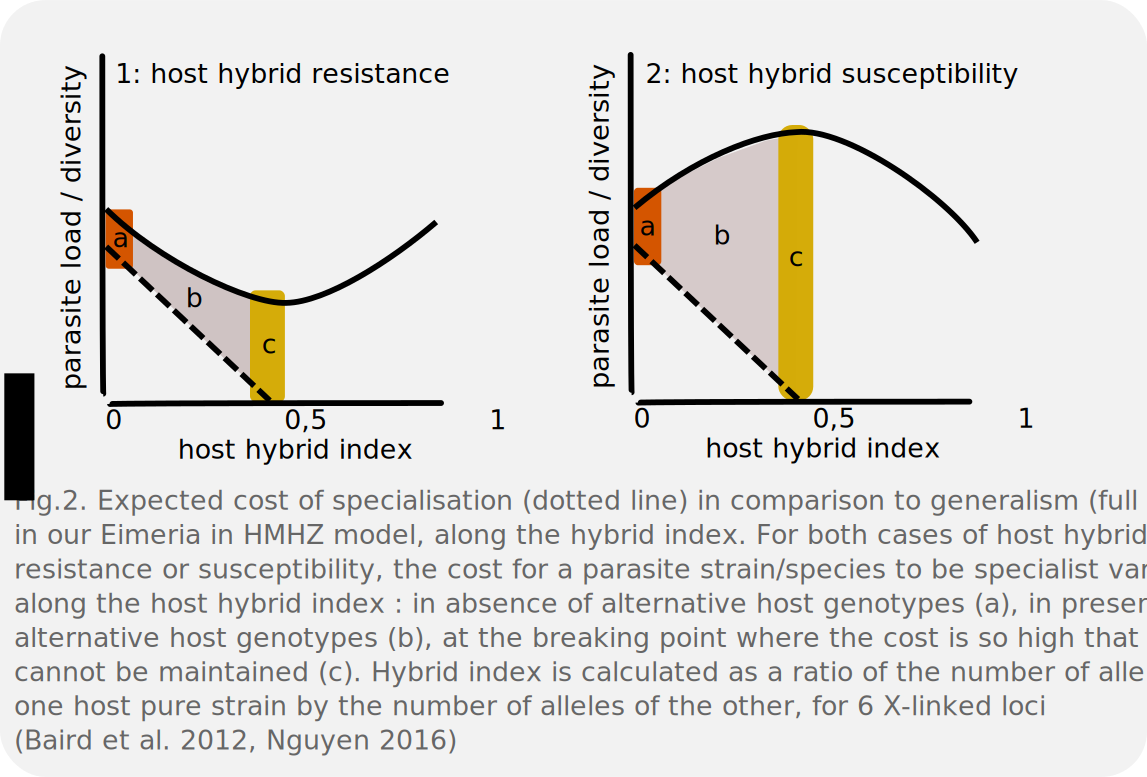
\includegraphics[scale=1]{Cost_specialist.png}
\end{center}
description

}

% PART II 
% -------

\block{Evidence of local adaptation}
{ Results of the infection experiment : 
  \begin{itemize}
    \item \textit{Eimeria} strain haplotype A  killed wild-derived mice at the beginning of the shedding period, regardless of mouse strain --> MORE?
    \item \textit{Eimeria} strain haplotype B has \textbf{lowest parasite shedding} in mice strains WSB compared to PWD, for a \textbf{highest relative weight loss} : evidence of \textbf{local adaptation}
    \item Mice hybrids lost less weight and  were less infected than the pure strains\\ \textbf{Possible hybrid vigor} (limitation : unknow effect of heterosis)\\
  \end{itemize}

  \begin{center}
  \includegraphics[scale=1.1]{May2017_E64.pdf}

  \end{center}
  
  some stats here!
}

\block{Perspective}
{
  \begin{center}
  \begin{itemize}
        \item Next cross infection experiment : verify our hypotheses (hybrid vigor, local adaptation), measure the effect of heterosis, add one parasite strains (another haplotype A, collected in the field)
        \item Analyse of divergence scenarios for \textit{Eimeria} spp. based on whole genomes and comparison of models of coalescence and cospeciations with their murine hosts (beyond the house mouse).
        \item Investigation of loci of coevolution, identifying parasite genes under divergent selection in the two house mouse subspecies. The coevolving loci corresponding on the host side will be investigated.
  \end{itemize}

%  \adjustbox{trim={.0\width} {.52\height} {0.0\width} {.0\height},clip}%
%		{\includegraphics[scale=1.4]{Figure_3.pdf}}
  \end{center}
}

% REFERENCES
% ----------

\block{References}
      {
        \begin{small}
          
          \hangindent=2cm Baird \textit{et al.} (2012) Where Are the Wormy Mice? A Reexamination of Hybrid Parasitism in the European House Mouse Hybrid Zone
           \textit{Evolution} 66 (9): 2757--72.

          \hangindent=2cm Jost (2016) Improvement of Genetic Markers and Phylogenetics of Eimeria Spp. from House Mouse
          Edited by Emanuel Heitlinger. \textit{Humboldt University}

          \hangindent=2cm Heitlinger \textit{et al.} (2014) The genome of Eimeria falciformis-reduction and specialization in a single host apicomplexan         parasite.\\ \textit{BMC genomics} 15 (1), 696
                    
          \hangindent=2cm Machol\'{a}n \textit{et al.} (2012) Evolution of the House Mouse
          \textit{Cambridge University Press}
          
        
          
        \end{small}
      }

      % ACKNOWLEDGEMENTS
% ----------------
      \note[targetoffsetx=-15cm, targetoffsety=-8cm, width=25cm, innersep=1cm]
{
    \begin{wrapfigure}{r}{3cm}	
    \vspace{-23pt}
	\includegraphics[scale=0.25]{Logos.png}
	
	\end{wrapfigure}
	\textbf{Funding:} This research has received funding 
	from the DFG, and is part of a IZW/HU project.
        A. Balard is part of the Dahlem Research School.
}


\end{columns}



% ----------------
\end{document}
\endinput
%%
%% End of file 